% The main focus of this chapter should be to introduce everything that is needed to understand the further concepts of the thesis.
% This should entail everything you had to learn to understand and implement the task, and shortly cover the courses in your specialization you needed to understand the topic.
% The goal is to enable a reader from the same study program potentially from another specialization to understand the thesis.
\chapter{Background}
\label{chap:background}

\begin{comment}
Kurse aus meiner Vertiefung:
- Prozessorarchitektur
- Funktionales Programmieren
- Grundlagen eingebetteter Systeme
- OS-based programming of embedded systems

- Real Time Linux (PREEMPT-RT specifically)
- hard vs soft real time
\end{comment}

There are several Prerequisites necessary for the rest of the thesis.
In this chapter we're first going to cover the architectural background of bare-metal, operating systems and scheduling,
then, continue with the language prerequisites for Rust and last, provide an overview of the hardware used.

\section{Bare-Metal vs Operating System}
\label{sec:background:bm_vs_os}

Many embedded systems run bare-metal, meaning without an operating system kernel that provides task scheduling, heap allocations and hardware access.
The reasons for this are that microcontrollers are often limit in their computational abilities and the operating system always causes some overhead.
In addition to the computational overhead many operating system scheduling strategies are optimized for throughput as opposed to reaction times.
With the event-driven nature of many embedded systems these higher and often unregular reaction times are not desireable.
As a result of this a specialized class of operating systems optimized for embedded systems exists.
These real time operating systems (RTOS) minimize the space and computation overhead and employ special scheduling strategies to guarantee worst-case reaction times.

While bare-metal systems have several advantages as already mentioned, they are not without their disadvantages.
Writing a bare-metal program requires the programmer to be closely familiar with several additional aspects of the project:
\begin{itemize}
    \item the hardware
    \begin{itemize}
        \item the processor and processor architecture the project is built for
        \item hardware interfaces and their protocols, such as SPI and PWM for our project
        \item understanding hardware interrupts may be required to write a performant implementation
    \end{itemize}
    \item the software
    \begin{itemize}
        \item many embedded platforms require a specific toolchain, that may come with its own caveats
        \item debugging is more complex and often requires the use of hardware interfaces such as JTAG
        \item hardware specific libraries
    \end{itemize}
\end{itemize}
All of these take additional time during a project and require more skilled programmers, which can add its own cost.

\subsection{Real time scheduling}
\label{sec:background:bm_vs_os:rtos}

Earlier we mentioned real time operating systems, but what does real time actually mean?
Real time systems are systems that guarantee the execution of a certain task before a certain time limit.


\subsection{PREEMP-RT}
\label{sec:background:bm_vs_os:preempt_rt}

\subsection{Circle}
\label{sec:background:bm_vs_os:circle}

\section{Rust Prerequisites}
\label{sec:background:rust}

Rust is a modern systems programming language,
that claims to achieve comparable performance to languages with manual managed memory such as C and C++,
while also being "memory safe", at term we will define more clearly shortly.
Many modern languages use a garbage collector to manage memory on the heap,
which is an additional thread that periodically checks all memory allocations to see if they are still used and frees them if they are not.
This introduces an overhead, as the main execution path may be interrupted by the garbage collector and the analysis of the existing alloction takes execution time.
Manually memory managed languages on the other hand suffer from the possibility of memory errors, such as double frees and use after frees.
Typically manually memory managed languages also allow for arbitrary memory access leading to data races, reading uninitialized memory, etc.
Rust aims to be the best of both worlds, managing memory without a garbage collector, while also avoiding memory management and access errors.

\subsection{Terminology}
\label{sec:background:terminology}

There are a few terms used in Rust that need only a short introduction.
First, a crate is the equivalent of a package in Rust, it can be either a library or an executable.
Second, traits are the equivalent of interfaces, we will use both terms interchangeably in this thesis.
Third, cargo is the build manager for Rust, comparable to NPM, CMake, Meson, Maven.

\subsection{Memory managment by ownership}
\label{sec:background:rust:ownership}

To achieve this Rust employs a combination of methods, the most important one being ownership.
Ownership in this context means that every resource has exactly one variable assigned as its owner.
For our purposes resource usually means "memory on the heap",
but can mean anything that needs setup and cleanup when it is used,
such as file descriptors, sockets, or an SPI connection.
The process of binding resource initialization and destruction to the lifetime of a variable is neither new,
nor an invention of Rust,
but rather the RAII (Resource acquisition is initialization) paradigm from C++.
Since in the real world resources need to be used from multiple points, Rust introduces three ways to safely allow that:
\begin{itemize}
    \item transferring ownership, called moving in Rust
    \item lending exclusive access, using a mutable reference
    \item sharing non-exclusive access, using multiple immutable references
\end{itemize}

Of these references, there can always only be either one mutable reference or an arbitrary number of immutable references per resource.
At compile time a part of the compiler called the borrow checker enforces this by checking the lifetimes of all references.
Reference lifetimes are their own complex topic and not necessary for the rest of this thesis, so we will not go into them.

\begin{lstlisting}[language=Rust,style=colouredRust]
// create a variable a that owns a heap allocation
let a = Box::new([0; 1000]);
// move the ownership from a to b
let b = a;
// this statement would now not compile, because a does not own the allocation anymore
let c = a[0];
\end{lstlisting}

\subsection{Unsafe Rust}
\label{sec:background:rust:unsafe}

Earlier we said that we'd define "memory safety" more closely, now is the time for that.
Operations in Rust are called memory unsafe when they cause undefined behavior (UB),
where undefined behavior is defined as the following by the \cite{Rustonomicon}:
\begin{itemize}
    \item Dereferencing dangling or unaligned pointers
    \item Breaking the pointer aliasing rules of LLVMs noalias memory model
    \item Calling a function with the wrong call ABI or unwinding from a function with the wrong unwind ABI
    \item Causing a data race
    \item Executing code compiled with target features that the current thread of execution does not support
    \item Producing invalid values:
          \begin{enumerate}
              \item a bool that isn't 0 or 1
              \item an enum with an invalid discriminant
              \item a null fn pointer
              \item a char outside the ranges [0x0, 0xD7FF] and [0xE000, 0x10FFFF]
              \item a ! (! is a type used to mark unreachable or infallible values)
              \item an integer (i*/u*), floating point value (f*), or raw pointer read from uninitialized memory, or uninitialized memory in a str
              \item a reference/Box that is dangling, unaligned, or points to an invalid value
              \item a wide reference, Box, or raw pointer that has invalid metadata:
                    \begin{itemize}
                        \item dyn Trait metadata is invalid if it is not a pointer to a vtable for Trait that matches the actual dynamic trait the pointer or reference points to
                        \item slice metadata is invalid if the length is not a valid usize
                    \end{itemize}
              \item a type with custom invalid values that is one of those values, such as a NonNull that is null.
          \end{enumerate}
\end{itemize}

This comes with a problem though, in order to prevent UB from occuring,
some operations such as reading from an arbitrary memory address are not possible,
because the compiler cannot check if the would cause UB.
But in reality there are cases where it is both necessary and safe to read from specific memory addressess,
most notably when talking to memory mapped IO.

This is where the unsafe keyword in Rust comes in.
Unsafe marks sections of code where the programmer has additional tools at his disposal, but is also responsible for upholding the aforementioned guarantees.
Unsafe code that successfully upholds all the invariants is called sound, unsafe code that can produce UB is called unsound.
The additional things unsafe allows us to do are:
\begin{itemize}
    \item Dereference raw pointers
    \item Call unsafe functions (including C functions, compiler intrinsics, and the raw allocator)
    \item Implement unsafe traits
    \item Mutate statics
    \item Access fields of unions
\end{itemize}

Most of these are uninteresting for us, so we will focus only on dereferencing raw pointers and calling unsafe functions.
Dereferencing raw pointers is self-explanatory in its meaning, the interesting part here is when is it sound to do so.
The pointer must be correctly aligned and not aliased.
If the access is a write we need to make sure that we don't cause data races through an additional read or write.

Calling other unsafe functions may not seem very important at a first glance,
but this changes, when we consider that there are a few sources of unsafe functions that are not written by us.
Most important for us are C functions.
Since C code is inherently memory unsafe it is up to the programmer to check its soundness.
So calling any C code from Rust needs to be done in an unsafe block.
The second important source of unsafe functions is in the standard library.
Here are compiler intrinsics, platform specific functions and raw access to the heap allocator, which allows for a C style manual memory management.

\subsection{Rust in the embedded world}
\label{sec:background:rust:embedded}

Since we will look at Rust through the lense of an embedded program, we should discuss the ecosystem around embedded programming in Rust.
When compared to C and C++ there is a notable amount of standardization in the Rust ecosystem.
The Rust Embedded SIG (Special Interest Group) provides several key libraries that provide common interfaces for all Rust embedded software to use.
This allows for a clear distinction between hardware drivers implementing these interfaces and using a generic version of the interface.
The most important of these libraries both in general and for our uses are:
\begin{itemize}
    \item embedded-hal (interfaces for SPI, PWM, I2C, GPIO, and delays)
    \item embedded-io (interfaces for UART, USB)
    \item critical-section (interafce for uninterrupted code execution)
\end{itemize}

There are also libraries for the CAN-bus, DMA controllers, and async versions of embedded-hal and embedded-io,
but, since these are not relevant for our project and function in similar ways to embedded-hal,
we will not discuss them further.

Implementations of these traits are called HALs (Hardware Abstraction Layers).
Typical implementations for a microcontroller consist of three parts:
\begin{enumerate}
    \item A Peripheral Access Crate (PAC) that contains all the memory addresses for the memory mapped IO. This can be generated using svd2rust from an svd file.
    \item A HAL crate that implements the embedded-hal traits, embedded-io traits for UART, DMA, PCIe and a critical section implementation for the bcm2711 processor.
    \item A Board Support Crate/Package (BSP) that contains board but not processor-specific implementations, such as the boot process, usb and ethernet.
\end{enumerate}

The svd2rust crate used for creating PACs is also an official crate maintained by the Embedded SIG.

\section{Hardware Details}
\label{sec:background:hardware}

With all the software details out of the way, we can take a closer look at the hardware that we'll be using.
First, we will give an overview over the Raspberry Pi and afterwards a detailed explanation of the parts we're actually using.
For communcation with our position encoder the iC-MU, we use the SPI bus and for sending the output signal to the motor driver, we use a PWM signal.

\subsection{Raspberry Pi 4}
\label{sec:background:hardware:pi}

The Raspberry Pi 4 is a Single Board Computer (SBC) based on the bcm2711 processor by Broadcom.
It has 4 64bit arm cores and current models run at a frequency of 1.8GHz, while earlier production units ran at 1.5GHz.
Interesting for us are mainly its IO capabilities.
The onboard GPIO pins support simple on/off input and output, as well as 6 SPI buses, 4 I2C buses, a UART port, and 2 PWM outputs.

\subsection{SPI}
\label{sec:background:hardware:spi}

The SPI bus is a serial communcation interface between one master and n slaves.
The name itself stands for "Serial Peripheral Interface".
It uses 4 lanes for communication\cite[p. 220]{SensornetzwerkeInTheorieUndPraxis}:

\begin{enumerate}
    \item CLK or SCLK - the clock generated by the master
    \item SS or CS or CE - of these lines there exists one per slave, it is used to select which slaves are currently enabled for communication. The names stand for "Slave Select", "Chip Select", "Chip Enable"
    \item MOSI or PICO - the data line which the master writes and the slaves read. The names stand for "Master out Slave in" and "Peripheral in Controller out"
    \item MISO or POCI - the data line which the slaves write and the master reads. The names stand for "Slave out Master in" and "Perihperal out Controller in"
\end{enumerate}

\begin{figure}[hp]
    \begin{center}
        \includesvg{assets/spi}
        \caption{Wiring of SPI with one master and two slaves}
        \label{fig:spi}
    \end{center}
\end{figure}

Depending on the polarity and phase of SCLK a SPI bus can be operated in four different modes.
The clock polarity is called CPOL and the clock phase CPHA.
A CPOL of $0$ means that SCLK idles at logical low and a CPOL of $1$ means that SCLK idles at logical high.
CPHA influences when data is sent.
When $CPHA = 0$ data is outputted when SCLK transitions to its idle level.
For $CPHA = 1$ data is outputted when SCLK transitions from its idle level.
The relation of CPOL and CPHA to the 4 Modes can be seen in table \ref{tab:spi_modes}.

\begin{table}[hp]
    \begin{tabular}{|l|l|l|}
        \hline
                 & CPOL = 0 & CPOL = 1 \\ \hline
        CPHA = 0 & Mode 0   & Mode 2   \\ \hline
        CPHA = 1 & Mode 1   & Mode 3   \\ \hline
    \end{tabular}
    \caption{SPI Modes}
    \label{tab:spi_modes}
\end{table}

\subsection{PWM}
\label{sec:background:hardware:pwm}

Since we're going to use PWM to control the motor driver, PWM should also get an introduction.
Pulse Width Modulation (PWM) is the technique of generating a digital signal where the ratio of on to off time is variable.
This allows to drive electric loads at only a percentage of their maximum power,
for example in dimming LEDs and running a motor at slower speeds.
The signal can be fully described by its frequency or period and duty-cycle or on-time.
The period is the time a full on-off cycle takes, the frequency simple the inverse.
The duty cycle and on-time describe what happens inside of a cycle,
with the duty cycle being the percentage of time that the signal is on and the on-time being the raw time value for which the signal is on.

\subsection{iC-MU}
\label{sec:background:hardware:ic-mu}

The iC-MU position encoder is a chip that is mounted on a motor in combination with a magnetic band in order to measure the current position of the motor,
as well as the number of previous rotations.
It is able to communicate this information through SPI, BiSS, SSI and ExtSSI.
Since the only common protocol with our Raspberry Pi is SPI, we use that.
The communication itself works by sending the chip an Opcode, optionally with some arguments such as a register address.
The chip replies by echoing the Opcode and any arguments and if applicable attaching the return values.
The different Opcodes are on byte long and can be seen in \ref{tab:opcodes}

\begin{table}[hp]
    \begin{tabular}{|l|l|}
        \hline
        Code & Description                     \\ \hline
        0xB0 & ACTIVATE                        \\ \hline
        0xA6 & SDAD-transmission (sensor data) \\ \hline
        0xF5 & SDAD Status                     \\ \hline
        0x97 & Read Register                   \\ \hline
        0xD2 & Write Register                  \\ \hline
        0xAD & Register Status                 \\ \hline
    \end{tabular}
    \caption{Opcodes for the iC-MU}
    \label{tab:opcodes}
\end{table}

The communication protocl the iC-MU expects is read from its configuration EEPROM and falls back to SPI.
Since all the default configuration values of the iC-MU are fine for us, we pulled the EEPROM data pin to ground.

The only OpCode we will use is the SDAD-transmission one, as it gets the current position of the motor.
The transmission process can be seen in \ref{fig:background:sdad}

\begin{figure}
    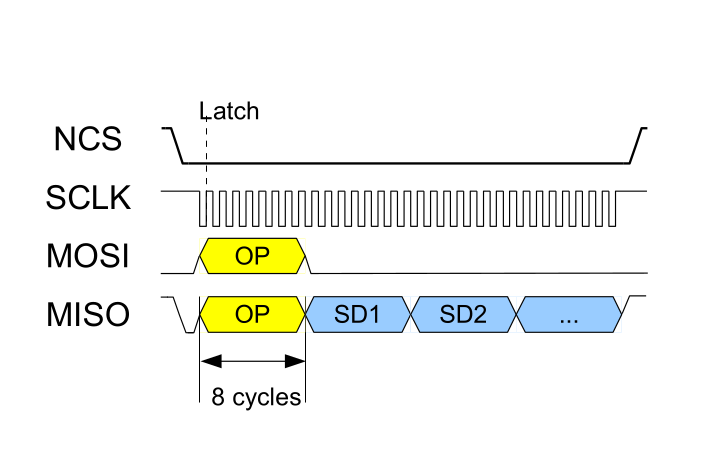
\includegraphics[width=.8\textwidth]{assets/sdad-transmission.png}
    \caption{}
    \label{fig:background:sdad}
\end{figure}
